\documentclass{article}\usepackage[]{graphicx}\usepackage[]{color}
%% maxwidth is the original width if it is less than linewidth
%% otherwise use linewidth (to make sure the graphics do not exceed the margin)
\makeatletter
\def\maxwidth{ %
  \ifdim\Gin@nat@width>\linewidth
    \linewidth
  \else
    \Gin@nat@width
  \fi
}
\makeatother

\definecolor{fgcolor}{rgb}{0.345, 0.345, 0.345}
\newcommand{\hlnum}[1]{\textcolor[rgb]{0.686,0.059,0.569}{#1}}%
\newcommand{\hlstr}[1]{\textcolor[rgb]{0.192,0.494,0.8}{#1}}%
\newcommand{\hlcom}[1]{\textcolor[rgb]{0.678,0.584,0.686}{\textit{#1}}}%
\newcommand{\hlopt}[1]{\textcolor[rgb]{0,0,0}{#1}}%
\newcommand{\hlstd}[1]{\textcolor[rgb]{0.345,0.345,0.345}{#1}}%
\newcommand{\hlkwa}[1]{\textcolor[rgb]{0.161,0.373,0.58}{\textbf{#1}}}%
\newcommand{\hlkwb}[1]{\textcolor[rgb]{0.69,0.353,0.396}{#1}}%
\newcommand{\hlkwc}[1]{\textcolor[rgb]{0.333,0.667,0.333}{#1}}%
\newcommand{\hlkwd}[1]{\textcolor[rgb]{0.737,0.353,0.396}{\textbf{#1}}}%
\let\hlipl\hlkwb

\usepackage{framed}
\makeatletter
\newenvironment{kframe}{%
 \def\at@end@of@kframe{}%
 \ifinner\ifhmode%
  \def\at@end@of@kframe{\end{minipage}}%
  \begin{minipage}{\columnwidth}%
 \fi\fi%
 \def\FrameCommand##1{\hskip\@totalleftmargin \hskip-\fboxsep
 \colorbox{shadecolor}{##1}\hskip-\fboxsep
     % There is no \\@totalrightmargin, so:
     \hskip-\linewidth \hskip-\@totalleftmargin \hskip\columnwidth}%
 \MakeFramed {\advance\hsize-\width
   \@totalleftmargin\z@ \linewidth\hsize
   \@setminipage}}%
 {\par\unskip\endMakeFramed%
 \at@end@of@kframe}
\makeatother

\definecolor{shadecolor}{rgb}{.97, .97, .97}
\definecolor{messagecolor}{rgb}{0, 0, 0}
\definecolor{warningcolor}{rgb}{1, 0, 1}
\definecolor{errorcolor}{rgb}{1, 0, 0}
\newenvironment{knitrout}{}{} % an empty environment to be redefined in TeX

\usepackage{alltt}

% Load required packages
\usepackage{amsmath, bm, booktabs, framed, hyperref, natbib}

\hypersetup{
    colorlinks=true,
    linkcolor=blue,
    citecolor=blue,
    urlcolor=blue
}

\bibliographystyle{plainnat}

% Define macros
\newcommand{\boot}{\ensuremath{^\star}}
\newcommand{\trans}{\ensuremath{^\top}}
\newcommand{\diag}{\operatorname{diag}}
\newcommand{\col}{\operatorname{col}}
\newcommand{\row}{\operatorname{row}}
\newcommand{\COV}{\operatorname{COV}}
\newcommand{\VAR}{\operatorname{VAR}}
\newcommand{\SE}{\operatorname{SE}}
\newcommand{\E}{\operatorname{E}}

\title{Inverse Estimation with Linear Mixed-Effects Models}
\author{Brandon M. Greenwell\\Infoscitex, a DCS company \\ and \\
        Christine M. Schubert Kabban\\Air Force Institute of Technology}
\date{\today}
\IfFileExists{upquote.sty}{\usepackage{upquote}}{}
\begin{document}

\maketitle




%%%%%%%%%%%%%%%%%%%%%%%%%%%%%%%%%%%%%%%%%%%%%%%%%%%%%%%%%%%%%%%%%%%%%%%%%%%%%%%%
% Abstract
%%%%%%%%%%%%%%%%%%%%%%%%%%%%%%%%%%%%%%%%%%%%%%%%%%%%%%%%%%%%%%%%%%%%%%%%%%%%%%%%

\begin{abstract}
Keep it to 200 words or less.
\end{abstract}


%%%%%%%%%%%%%%%%%%%%%%%%%%%%%%%%%%%%%%%%%%%%%%%%%%%%%%%%%%%%%%%%%%%%%%%%%%%%%%%%
\section{Introduction}
%%%%%%%%%%%%%%%%%%%%%%%%%%%%%%%%%%%%%%%%%%%%%%%%%%%%%%%%%%%%%%%%%%%%%%%%%%%%%%%%

This paper concerns inverse estimation with linear mixed-effects models (LMMs). Consider an ordinary regression model $\mathcal{Y}_i = f\left(x_i; \bm{\beta} \right) + \epsilon_i$ $(i = 1, \dotsc, n)$, where $f$ is a known expectation function (called a \emph{calibration curve}) that is monotonic over the range of interest and $\epsilon_i \stackrel{iid}{\sim} \mathcal{N}\left( 0, \sigma^2 \right)$.  A common problem in regression is to predict a future response $\mathcal{Y}_0$ (or estimate the mean response $f_0 = \E\left[\mathcal{Y}_0\right]$) for a known value of the explanatory variable $x_0$.  Often, however, there is a need to do the reverse; that is, given an observed value of the response $\mathcal{Y} = y_0$ (or a specified value of the mean response), infer the unknown value of the explanatory variable $x_0$.  This is known as the \emph{calibration problem}, though we refer to it more generally as inverse estimation.  A thorough overview of the calibration problem is given in \citet{osborne-statistical-1991}.  \citet{oman-calibration-1998} considers the case of a random intercept and slope model. 

The majority of literature on inverse estimation, however, concerns \textit{cross-sectional data}---?. In this paper, we expand this to the case of \textit{dependent data} (e.g., \textit{longitudinal data} or \textit{repeated measures data}). Analyzing these types of data is more theoretically challenging, but fortunately, modern day computers and algorithms make this a rather simple task.

In Section~\ref{sec:point}, we extend the classical inverse estimate. Section~\ref{sec:wald} and Section~\ref{sec:inversion} discuss approximate interval estimates by extending the classical Wald and inversion methods, respectively. Section~\ref{sec:boot} introduces a fully parametric bootstrap algorithm for making inference on $x_0$. 




%%%%%%%%%%%%%%%%%%%%%%%%%%%%%%%%%%%%%%%%%%%%%%%%%%%%%%%%%%%%%%%%%%%%%%%%%%%%%%%%
\section{Linear mixed-effects models}
\label{sec:lmm}
%%%%%%%%%%%%%%%%%%%%%%%%%%%%%%%%%%%%%%%%%%%%%%%%%%%%%%%%%%%%%%%%%%%%%%%%%%%%%%%%

Linear regression models with random coefficients can be represented in many different (but equivalent) forms.  One of the most common forms, attributed to \citet{laird-random-1982}, is
\begin{equation}
\label{eqn:lmm-laird-and-ware}
  \bm{\mathcal{Y}}_i = \bm{X}_i\bm{\beta} + \bm{Z}_i\bm{b}_i + \bm{\epsilon}_i, \quad i = 1, \dotsc, m,
\end{equation}
where
\begin{itemize}
  \item $\bm{\mathcal{Y}}_i$ is an $n_i \times 1$ response vector for the $i$-th subject/cluster/group;
  \item $\bm{X}_i$ is an $n_i \times p$ design matrix for the fixed-effects;
  \item $\bm{Z}_i$ is an $n_i \times q$ design matrix for the random-effects;
  \item $\bm{\beta}$ is a $p \times 1$ vector of fixed-effects coefficients;
  \item $\bm{b}_i$ is a $q \times 1$ vector of random-effects coefficients with mean zero and variance-covariance matrix $\bm{D}$;
  \item $\bm{D}$ is a $q \times q$ variance-covariance matrix for the random-effects;
  \item $\bm{\epsilon}_i$ is an $n_i \times 1$ vector of random errors with mean zero and variance-covariance matrix $\sigma^2\bm{I}$.
\end{itemize}
Equation~\eqref{eqn:lmm-laird-and-ware} is known as a linear mixed-effects model (LMM).  The random-effects and errors are often assumed to follow a normal distribution.  By stacking the data, the (normal) LMM can be written concisely as
\begin{equation}
\label{eqn:lmm-stacked}
    \bm{\mathcal{Y}} = \bm{X}\bm{\beta} + \bm{Z}\bm{b} + \bm{\epsilon}, \quad
      \begin{bmatrix}
        \bm{b} \\
        \bm{\epsilon}
      \end{bmatrix} \sim
      \mathcal{N}\left(\begin{bmatrix}
        \bm{0} \\
        \bm{0}
      \end{bmatrix}, \begin{bmatrix}
        \bm{D} & \bm{0} \\
        \bm{0} & \sigma^2\bm{I}
      \end{bmatrix}\right),
\end{equation}
where $\bm{\mathcal{Y}} = \col\left\{\bm{\mathcal{Y}}_i\right\}$, $\bm{X} = \col\left\{\bm{X}_i\right\}$, $\bm{Z} = \diag\left\{\bm{Z}_i\right\}$, $\bm{b} = \col\left\{\bm{b}_i\right\}$, and $\bm{\epsilon} = \col\left\{\bm{\epsilon}_i\right\}$ for $i = 1, \dotsc, m$.  Since $\COV\left[\bm{b}, \bm{\epsilon}\right] = \bm{0}$, it is assumed that the random vectors $\big\{ \bm{b}_i, \bm{\epsilon}_i \big\}_{i=1}^m$ are mutually independent.

The additional term $\bm{Z}\bm{b}$ in the model imposes a specific variance-covariance structure on the response vector $\bm{\mathcal{Y}}$:
\[
  \bm{\mathcal{Y}} \sim \mathcal{N}\left(\bm{X}\bm{\beta}, \bm{V}\right), \quad \bm{V} = \bm{Z}\bm{D}\bm{Z}\trans + \sigma^2\bm{I}.
\]
Thus, the fixed-effects determine the mean of $\bm{\mathcal{Y}}$, while the random-effects govern the variance-covariance structure of $\bm{\mathcal{Y}}$.  Different random-effects structures impose different variance-covariance structures on the response resulting in a highly flexible framework for modelling \emph{grouped data}.

The random-effects variance-covariance matrix $\bm{D}$ has at most $q(q+1)/2$ unique elements which we represent by the vector $\bm{\theta}$.  There are a number of methods available for estimating $\left( \bm{\beta}, \sigma^2, \bm{\theta} \right)$; see, for example, \citet[chap 6.]{mcculloch_generalized_2008} and \citet[chap. 2]{demidenko_mixed_2013}.  Most commonly, the fixed-effects $\bm{\beta}$ are estimated via the method of maximum likelihood (ML), while the variance components $\left(\sigma^2, \bm{\theta}\right)$ are estimated via restricted maximum likelihood (REML).  The ML estimator of $\bm{\beta}$, given by
\begin{equation*}
\widehat{\bm{\beta}} = \left( \bm{X}\trans \widehat{\bm{V}}^{-1} \bm{X} \right)\bm{X}\trans\bm{\mathcal{Y}},
\end{equation*}
depends on the estimated variance components through $\widehat{\bm{V}}$ which makes it difficult to capture the variability of $\widehat{\bm{\beta}}$ in small sample sizes (see \citet[pp. 165-167]{mcculloch_generalized_2008}).  The usual practice is to ignore the variability of the estimated variance components when making inference about the fixed-effects; that is, treat $\widehat{\bm{V}}$ as the true (fixed) value of $\bm{V}$.  Modern computational procedures such as the parametric bootstrap and Markov chain Monte Carlo (MCMC) methods are two ways account for the variability of the estimated variance components.


%%%%%%%%%%%%%%%%%%%%%%%%%%%%%%%%%%%%%%%%%%%%%%%%%%%%%%%%%%%%%%%%%%%%%%%%%%%%%%%%
\subsection{Bladder volume data}
%%%%%%%%%%%%%%%%%%%%%%%%%%%%%%%%%%%%%%%%%%%%%%%%%%%%%%%%%%%%%%%%%%%%%%%%%%%%%%%%

For illustration, let us consider the bladder volume data which can be found in \citet[pg. 7]{brown-measurement-1993} and \citet{oman-calibration-1998}.  In Brown's words:
\begin{quotation}
\noindent``A series of 23 women patients attending a urodynamic clinic were recruited for the study. After successful voiding of the bladder, sterile water was introduced in additions of 1, 1.5, and then 2.5 cl increments up to a final cumulative total of 17.5 cl. At each volume a measure of height (\texttt{H}) in mm and depth (\texttt{D}) in mm of largest ultrasound bladder images were taken. The product \texttt{H} $\times$ \texttt{D} was taken as a measure of liquid volume.''
\end{quotation}
We took Brown's suggestion and transformed the data so that the relationship is approximately linear.  Spaghetti plots of both the original and transformed data are displayed in Figure~\ref{fig:spaghetti}.

\begin{knitrout}
\definecolor{shadecolor}{rgb}{0.969, 0.969, 0.969}\color{fgcolor}\begin{figure}[!htb]
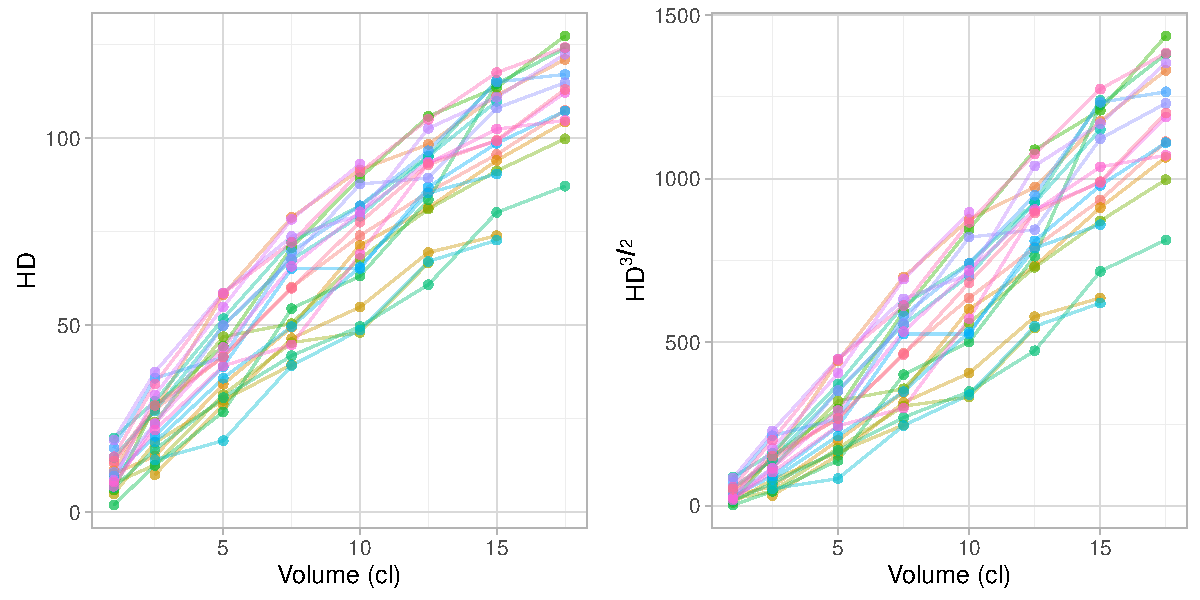
\includegraphics[width=\linewidth]{figure/spaghetti-1} \caption{Spaghettiplot of bladder volume data (lines connect measurements belonging to the same subject). \textit{Left}: Original data. \textit{Right}: Transformed data.}\label{fig:spaghetti}
\end{figure}


\end{knitrout}

A random intercept and slope model with uncorrelated random-effects fits the transformed data (right side of Figure~\ref{fig:spaghetti}) well:
\begin{align*}
  \texttt{HD}^{3/2}_{ij} &= \left(\beta_0 + b_{0i}\right) + \left(\beta_1 + b_{1i}\right)\texttt{volume}_{ij} + \epsilon_{ij} \\
  b_{ki} &\sim \mathcal{N}\left(0, \theta_k^2\right), \quad k = 0, 1, \\
  \epsilon_{ij} &\sim \mathcal{N}\left(0, \sigma^2\right),
\end{align*}
where $\COV\left[b_{0i}, b_{1i}\right] = 0$.  Table~\ref{tab:transformed-lmm} displays the fixed-effects results from applying this model to the transformed bladder volume data. %To fit such a model in \texttt{R}, we can use the recommended \texttt{nlme} package \citep{pinheiro-nlme-2013}:



\begin{table}
\begin{tabular}{lrrrrr}
  \hline
  Parameter & Value   & Std.Error & DF  & $t$-value & $p$-value\\
  \hline
  intercept & -53.832 & 11.603    & 142 & -4.639    & $<0.001$\\
  volume    & 69.095  & 3.114     & 142 & 22.191    & $<0.001$\\
  \hline
  \end{tabular}
  \caption{Output for fixed-effects portion of LMM fit to the transformed bladder volume data.} 
  \label{tab:transformed-lmm}
\end{table}

%The \texttt{pdDiag} function forces a diagonal variance-covariance structure on the random-effects; hence, a covariance of zero. The same model, but with an additional quadratic term, provides a useful fit to the original data (left side of Figure~\ref{fig:spaghetti}):
% \begin{align*}
%   \texttt{HD}_{ij} &= \left(\beta_0 + b_{0i}\right) + \left(\beta_1 + b_{1i}\right)\texttt{volume}_{ij} + \beta_2\texttt{volume}_{ij}^2 + \epsilon_{ij} \\
%   b_{ki} &\sim \mathcal{N}\left(0, \theta_k^2\right), \quad k = 0, 1, \\
%   \epsilon_{ij} &\sim \mathcal{N}\left(0, \sigma^2\right).
% \end{align*}
For an in-depth treatment on fitting LMMs using the \texttt{nlme} software, see \citet{pinheiro-mixed-2000}.


%%%%%%%%%%%%%%%%%%%%%%%%%%%%%%%%%%%%%%%%%%%%%%%%%%%%%%%%%%%%%%%%%%%%%%%%%%%%%%%%
% Point estimation
%%%%%%%%%%%%%%%%%%%%%%%%%%%%%%%%%%%%%%%%%%%%%%%%%%%%%%%%%%%%%%%%%%%%%%%%%%%%%%%%

\section{Point estimation}\label{sec:point}

The standard methods of calibration, (i.e., the Wald-based and inversion confidence intervals) are easily extended to the case of random coefficients.  For convenience, let us write the linear random coefficient model as
\begin{equation*}
  \mathcal{Y}_{ij} = f\left(x_{ij}; \bm{\beta}\right) + R\left(x_{ij}; \bm{b}_i\right) + \epsilon_{ij},
\end{equation*}
where $f(\cdot)$ and $R(\cdot)$ are linear in $\bm{\beta}$ and $\bm{b}_i$, respectively.  For instance, the model for the transformed bladder data has $f\left(\texttt{volume}_{ij}; \bm{\beta}\right) = \beta_0 + \beta_1 \texttt{volume}_{ij}$ and $R\left(\texttt{volume}_{ij}; \bm{b}_i\right) = b_{0i} + b_{1i}\texttt{volume}_{ij}$ with $\E\left[R\left(\texttt{volume}_{ij}; \bm{b}_i\right)\right] = 0$ and $\VAR\left[R\left(\texttt{volume}_{ij}; \bm{b}_i\right)\right] = \theta_0^2 + \texttt{volume}_{ij}^2\theta_1^2$.

Assume that, after the data are collected and a model is fitted, we obtain a new observation, denoted $\mathcal{Y}_0$, from the same population under study for which the value of the explanatory variable $x_0$ is unknown.  We assume that the new observation belongs to a group not included in our analysis.  Estimating $x_0$ is rather straightforward.  By assumption, the new observation $\mathcal{Y}_0$ is distributed as a $\mathcal{N}\left\{f\left(x_0; \bm{\beta}\right), \sigma_0^2\right\}$ random variable with $\sigma_0^2 = \VAR\left[ R\left( x_0; \bm{b}_0 \right) \right ] + \sigma^2$.  A natural estimator for $x_0$ is then
\begin{equation}
\label{eqn:est}
  \widehat{x}_0 = f^{-1}\left(\mathcal{Y}_0; \widehat{\bm{\beta}}\right),
\end{equation}
where $\widehat{\bm{\beta}}$ is the ML estimator of $\bm{\beta}$.  We shall refer to Equation~\eqref{eqn:est} as the classical estimator.  Note that the point estimate $\widehat{x}_0$ does not involve any of the random-effects; the random-effects only contribute to the variance-covariance structure of the response.


%%%%%%%%%%%%%%%%%%%%%%%%%%%%%%%%%%%%%%%%%%%%%%%%%%%%%%%%%%%%%%%%%%%%%%%%%%%%%%%%
% Wald interval
%%%%%%%%%%%%%%%%%%%%%%%%%%%%%%%%%%%%%%%%%%%%%%%%%%%%%%%%%%%%%%%%%%%%%%%%%%%%%%%%

\section{Wald interval}\label{sec:wald}

An approximate $100(1-\alpha)\%$ Wald-type confidence interval for $x_0$ has the simple form
\begin{equation}
\label{eqn:wald}
  CI_{wald}\left(x_0\right) = \left( \widehat{x}_0 -  \SE\left[\widehat{x}_0\right]\Phi\left(\alpha/2\right),  \widehat{x}_0 -  \SE\left[\widehat{x}_0\right]\Phi\left(1-\alpha/2\right) \right).
\end{equation}
There is no ``textbook'' formula for the standard error of $\widehat{x}_0$---not even in the case of the simple linear regression model. Instead, an estimate of the standard error is obtained using a first-order Taylor series approximation, or better yet, a bootstrap approximation.  

The Taylor series approximation relies on the variance-covariance matrix of $\left(\mathcal{Y}_0, \widehat{\bm{\beta}}\right)$, namely,
\[
\Sigma = \begin{bmatrix}
           \VAR\left[\mathcal{Y}_0\right] & \bm{0} \\
           \bm{0} & \VAR\left[\widehat{\bm{\beta}}\right]
         \end{bmatrix} = \begin{bmatrix}
           \sigma_0^2 & \bm{0} \\
           \bm{0} & \left(\bm{X}\trans\bm{V}^{-1}\bm{X}\right)^{-1}
         \end{bmatrix}.
\]
Since $\mathcal{Y}_0$ is independent of $\bm{\mathcal{Y}}$, it is also independent of $\widehat{\bm{\beta}}$, hence the diagonal structure of $\Sigma$. Recall that our point estimate has the form $x = f^{-1}\left(y; \bm{\beta}\right)$. Let $f_1^{-1}\left(y; \bm{\beta}\right)$ and $f_2^{-1}\left(y; \bm{\beta}\right)$ denote the partial derivatives of $f^{-1}$ with respect to the parameters $y$ and $\bm{\beta}$, respectively. Our point estimator is given by $f^{-1}\left(\mathcal{Y}_0; \widehat{\bm{\beta}}\right)$, where $\mathcal{Y}_0$ is a new observation and $\widehat{\bm{\beta}}$ is the ML estimator of $\bm{\beta}$.  A first-order Taylor-series approximation for the variance of $\widehat{x}_0$ is given by
\begin{align}
  \VAR\left[\widehat{x}_0\right] &= \left[f_1^{-1}\left(\mathcal{Y}_0; \widehat{\bm{\beta}}\right)\right]^2\sigma_0^2 \nonumber \\
   &+ \left[f_2^{-1}\left(\mathcal{Y}_0; \widehat{\bm{\beta}}\right)\right]\trans\left(\bm{X}\trans\bm{V}^{-1}\bm{X}\right)^{-1}\left[f_2^{-1}\left(\mathcal{Y}_0; \widehat{\bm{\beta}}\right)\right].
\end{align}
To obtain $\SE\left[\widehat{x}_0\right] = \Big\{ \widehat{\VAR}\left[\widehat{x}_0\right] \Big\}^{1/2}$, we simply replace $\sigma_0^2$ and $\bm{V}$ with their respective estimates $\widehat{\sigma}_0^2$ and $\widehat{\bm{V}}$.

The Wald-based interval is simple to compute as long as we have an estimate for the standard error. As we will discuss in Section~\ref{sec:R}, the \texttt{R} package \texttt{investr} \citep{investr-package} can be used to obtain the Wald-based interval \eqref{eqn:wald} using a Taylor series approximation of the standard error. If a closed-form formula is available for $\widehat{x}_0$, then the \texttt{deltaMethod} function from the \texttt{car} package \citep{fox-car-2011} can also be used to obtain the Taylor series approximation of the standard error. Alternatively, one can use the parametric bootstrap instead of relying on a Taylor series approximation; see Section~\ref{sec:boot}. The bootstrap estimate may be more accurate in smaller sample sizes because, unlike the Taylor approximation estimate, it takes into account the variability of the estimated variance components. The \texttt{bootMer} function in the \texttt{lme4} package \citep{bates-lme4-2014} can be used for model-based parametric bootstrapping in mixed-effects models.


%%%%%%%%%%%%%%%%%%%%%%%%%%%%%%%%%%%%%%%%%%%%%%%%%%%%%%%%%%%%%%%%%%%%%%%%%%%%%%%%
% Inversion interval
%%%%%%%%%%%%%%%%%%%%%%%%%%%%%%%%%%%%%%%%%%%%%%%%%%%%%%%%%%%%%%%%%%%%%%%%%%%%%%%%

\section{Inversion interval}\label{sec:inversion}

In the case of the simple linear regression model with constant variance, an exact $100(1-\alpha)\%$ confidence interval for $x_0$ can be derived \citep{graybill-theory-1976}.  This can be generalized to an approximate method in the case of polynomial or nonlinear regression models with independent observations and constant variance (see \citet{seber-nonlinear-2003} and \citet{huet-statistical-2004}).  In a similar fashion, we can generalize the same results to an approximate method for linear mixed-effects models.  

Let $\widehat{f}_0 = f\left(x_0; \widehat{\bm{\beta}}\right)$ be the predicted mean at $x = x_0$.  A prediction interval for $\mathcal{Y}_0$ at $x_0$ with asymptotic coverage probability $100(1-\alpha)\%$ is
\begin{equation}
\label{eqn:asymptotic-pi}
  \mathcal{I}_\infty\left(x_0\right) = \widehat{f}_0 \pm z_{1-\alpha/2}\left\{ \widehat{\VAR}\left[\mathcal{Y}_0 - \widehat{f}_0\right] \right\}^{1/2}.
\end{equation}
If instead, $\mathcal{Y}_0$ is observed to be $y_0$ and $x_0$ is unknown, then an asymptotic $100(1-\alpha)\%$ confidence interval for the unknown $x_0$ can be obtained by inverting \eqref{eqn:asymptotic-pi}:
\begin{equation}
\label{eqn:inversion}
  CI_{inv}\left(x_0\right) = \left\{ x: z_{\alpha/2} \le \frac{\mathcal{Y}_0-f\left(x; \widehat{\bm{\beta}}\right)}{\left\{ \widehat{\VAR}\left[\mathcal{Y}_0 - f\left(x; \widehat{\bm{\beta}}\right)\right] \right\}^{1/2}} \le z_{1-\alpha/2} \right\}.
\end{equation}
This is known as the \emph{inversion interval} and typically cannot be written in closed-form; therefore, numerical techniques are required to find the lower and upper bounds.  Further, note that $CI_{inv}\left(x_0\right)$ is not symmetric about $\widehat{x}_0$ and will not necessarily result in a single finite interval.

Fortunately, the inversion interval \eqref{eqn:inversion} can be computed automatically using the \texttt{investr} package.  However, like the Wald-based interval \eqref{eqn:wald}, the inversion interval ignores the variability of the estimated variance components and will likely perform poorly in small sample sizes.  An alternative approach involving the parametric bootstrap will be discussed in Section~\ref{sec:boot}.

Finally, the inversion interval uses a normal approximation.  While it is likely that a $t$-distribution may be more accurate, it is difficult to find the appropriate degrees of freedom. \citet{oman-calibration-1998}, suggests a $t$-distribution with $N-1$ degrees of freedom ($N$ being the total sample size).


%%%%%%%%%%%%%%%%%%%%%%%%%%%%%%%%%%%%%%%%%%%%%%%%%%%%%%%%%%%%%%%%%%%%%%%%%%%%%%%%
% Parametric bootstrap
%%%%%%%%%%%%%%%%%%%%%%%%%%%%%%%%%%%%%%%%%%%%%%%%%%%%%%%%%%%%%%%%%%%%%%%%%%%%%%%%

\section{Parametric bootstrap}\label{sec:boot}

The bootstrap \citep{efron-bootstrap-1979} is a general-purpose computer-based method for assessing accuracy of estimators and forming confidence intervals for parameters.  \citet{jones-bootstrapping-1999} proposed a nonparametric bootstrap algorithm for controlled calibration with independent observations.  However, since our application involves random coefficients (i.e., dependent observations), the nonparametric bootstrap does not easily apply, and instead, we adopt a ``fully parametric'' approach.  In a parametric bootstrap, bootstrap samples are generated from a fitted parametric model rather than sampling with replacement directly from the data.  Fortunately, parametric bootstrap confidence intervals are usually more accurate than nonparametric ones, however, by sampling from a fitted parametric family, we are implicitly assuming that we have the ``correct model''.

Let $\widehat{\sigma}_0^2$ be an estimate of the variance of the new observation $\mathcal{Y}_0$.  An algorithm for bootstrapping $\widehat{x}_0$ in an LMM is given in Figure~\ref{fig:parboot}.  Note that step 5. is crucial for calibration problems because we need to treat $y_0$ as a random quantity in the bootstrap simulation, otherwise the variability of $\widehat{x}_0$ will be underestimated; see, for example, \citet{jones-bootstrapping-1999} and \citet{greenwell-investr-2014}.
\begin{figure}[!htb]
\begin{enumerate}
  \item Fit a mixed model \eqref{eqn:lmm-stacked} to the data and obtain estimates $\widehat{\bm{\beta}}$, $\widehat{\bm{D}}$, and $\widehat{\sigma}^2$.
	\item Define $\bm{y}\boot = \bm{X}\widehat{\bm{\beta}} + \bm{Z}\bm{b}\boot + \bm{\epsilon}\boot$, where $\bm{b}\boot \sim \mathcal{N}_q\left(\bm{0}, \widehat{\bm{D}}\right)$ and $\bm{\epsilon}\boot \sim \mathcal{N}_N\left(\bm{0}, \widehat{\sigma}_\epsilon^2\bm{I}\right)$;
	\item Update the original model using $\bm{y}\boot$ as the response vector to obtain $\widehat{\bm{\beta}}\boot$ and $\widehat{\sigma}_0^{2\star}$;
	\item Generate $y_0\boot \sim \mathcal{N}\left(y_0, \widehat{\sigma}_0^{2\star}\right)$;
	\item Define $\widehat{x}_0\boot = f^{-1}\left(y_0\boot; \widehat{\bm{\beta}}\boot\right)$;
  \item Repeat steps (2)-(5) $R$ times.
\end{enumerate}
\caption{Parametric bootstrap algorithm for linear calibration with random coefficients. \label{fig:parboot}}
\end{figure}

There are three main bootstrap confidence interval procedures: The percentile methods introduced in \citet{efron-bootstrap-1979}, the studentized bootstrap $t$ method introduced in \citet{efron-jackknife-1982}, and the double bootstrap method \citep{hall-bootstrap-1986}. For a good overview of all these confidence interval procedures, see \citet[chap. 5]{hinkley-bootstrap-1997} and \citet[chap. 11]{boos-essential-2013}. In the next section, we discuss how to use this algorithm to adjust the previously discussed inversion interval.


% %%%%%%%%%%%%%%%%%%%%%%%%%%%%%%%%%%%%%%%%%%%%%%%%%%%%%%%%%%%%%%%%%%%%%%%%%%%%%%%%
% \subsection{A bootstrap percentile interval for $x_0$}
% %%%%%%%%%%%%%%%%%%%%%%%%%%%%%%%%%%%%%%%%%%%%%%%%%%%%%%%%%%%%%%%%%%%%%%%%%%%%%%%%
% 
% The percentile method is the simplest and is given by the sample $\alpha/2$ and $1-\alpha/2$ quantiles of the bootstrap sample.  Let $\widehat{x}_{1*}, \dotsc, \widehat{x}_{R*}$ be a bootstrap sample obtained from the algorithm in Figure~\ref{fig:parboot}.  If $\widehat{F}_R$ is the empirical distribution function of the bootstrap sample, then an approximate $100(1-\alpha)\%$ confidence interval for $x_0$ is given by
% \[
%   \left( \widehat{F}_R^{-1}(\alpha/2), \widehat{F}_R^{-1}(1-\alpha/2) \right).
% \]
% The percentile interval is transformation respecting; thus, if we want a confidence interval for any one-to-one transformation $g\left(\widehat{x}_0\right)$, then we can just apply the transformation to the endpoints of the percentile interval for $\widehat{x}_0$.  The drawback is that the percentile interval is only \emph{first-order accurate} (see \citet[pp. 429-430]{boos-essential-2013}).  \citet{efron-better-1987} offered an improvement over the percentile interval called the \emph{bias-corrected and accelerated} ($BC_a$) interval that often obtains second-order accuracy and is transformation respecting.  However, the recommended \texttt{R} package \texttt{boot} \citep{canty-boot-2013} we will be relying on currently does not allow for $BC_a$ confidence intervals to be constructed from a parametric bootstrap.
% 
% 
% %%%%%%%%%%%%%%%%%%%%%%%%%%%%%%%%%%%%%%%%%%%%%%%%%%%%%%%%%%%%%%%%%%%%%%%%%%%%%%%%
% \subsection{A bootstrap $t$ interval for $x_0$}
% %%%%%%%%%%%%%%%%%%%%%%%%%%%%%%%%%%%%%%%%%%%%%%%%%%%%%%%%%%%%%%%%%%%%%%%%%%%%%%%%
% 
% A bootstrap $t$ interval for $x_0$ is essentially a bootstrap adjusted Wald-type interval.  The Wald interval for $x_0$ \eqref{eqn:wald} assumes that
% \[
%   Q_W = \frac{\widehat{x}_0 - x_0}{\SE\left[\widehat{x}_0\right]} \sim \mathcal{N}(0, 1).
% \]
% Rather than assuming that $Q_W$ is normal, the bootstrap $t$ method uses the bootstrap distribution of $Q_W\boot = \left(\widehat{x}_0\boot - \widehat{x}_0\right)/\SE\left[\widehat{x}_0\boot\right]$ to estimate the true distribution of $Q_W$.  If $\widehat{F}_{Q_W}$ is the empirical distribution function for a sample of $R$ bootstrap replicates of $Q_W$, then the bootstrap $t$  interval for $x_0$ is given by
% \[
%     CI_{wald}\boot\left(x_0\right) = \left( \widehat{x}_0 -  \SE\left[\widehat{x}_0\right]\widehat{F}_{Q_W}\left(\alpha/2\right),  \widehat{x}_0 -  \SE\left[\widehat{x}_0\right]\widehat{F}_{Q_W}\left(1-\alpha/2\right) \right).
% \]
% In order to implement this method, we need to calculate the standard error of each bootstrap replicate.  To do this, we can either use an additional (nested) bootstrap to estimate the standard error, or use a Taylor series approximation as discussed in Section~\ref{sec:wald}.  If time is  not a factor, then the nested bootstrap is preferred since bootstrap standard errors are usually more accurate than those based on a first-order Taylor series approximation \citep[pp. 478-480]{casella-statistical-2002}.  The benefits of using this interval over \eqref{eqn:wald} are that (a) it does not assume normality (hence, likely to be more accurate in smaller sample sizes) and (b) it is not symmetric about $\widehat{x}_0$; thus, more realistic when the response is nonlinear in $x$ (e.g., polynomials, etc.).


%%%%%%%%%%%%%%%%%%%%%%%%%%%%%%%%%%%%%%%%%%%%%%%%%%%%%%%%%%%%%%%%%%%%%%%%%%%%%%%%
\subsection{A bootstrap adjusted inversion interval for $x_0$}
%%%%%%%%%%%%%%%%%%%%%%%%%%%%%%%%%%%%%%%%%%%%%%%%%%%%%%%%%%%%%%%%%%%%%%%%%%%%%%%%

\citet{huet-statistical-2004} suggests a bootstrap modification of the usual inversion interval in nonlinear regression models with dependent data.  In a similar fashion, we could use the parametric bootstrap to adjust the approximate inversion interval given in Equation~\eqref{eqn:inversion}.  The inversion interval assumes that the \emph{predictive pivot}
\[
  Q_I = \frac{\mathcal{Y}_0-f\left(x; \widehat{\bm{\beta}}\right)}{\left\{ \widehat{\VAR}\left[\mathcal{Y}_0 - f\left(x; \widehat{\bm{\beta}}\right)\right] \right\}^{1/2}} \sim \mathcal{N}(0, 1).
\]
A bootstrap modified inversion interval would then use the bootstrap distribution of
\[
  Q_I\boot = \frac{\mathcal{Y}_0\boot-f\left(\widehat{x}_0; \widehat{\bm{\beta}}\boot\right)}{\left\{ \widehat{\VAR}\left[\mathcal{Y}_0 - f\left(\widehat{x}_0; \widehat{\bm{\beta}}\boot\right)\right] \right\}^{1/2}},
\]
to estimate the true distribution of $Q_I$.  If $\widehat{F}_{Q_I}$ is the empirical distribution function for a sample of $R$ bootstrap replicates of $Q_I$, then the modified inversion interval for $x_0$ is given by
\[
    CI_{inv}\boot\left(x_0\right) = \left\{ x: \widehat{F}_{Q_I}\left(\alpha/2\right) \le Q_I \le \widehat{F}_{Q_I}\left(1-\alpha/2\right) \right\}.
\]
\vspace{25pt}


% %%%%%%%%%%%%%%%%%%%%%%%%%%%%%%%%%%%%%%%%%%%%%%%%%%%%%%%%%%%%%%%%%%%%%%%%%%%%%%%%
% \section{An objective Bayesian approach}
% \label{sec:bayesian}
% %%%%%%%%%%%%%%%%%%%%%%%%%%%%%%%%%%%%%%%%%%%%%%%%%%%%%%%%%%%%%%%%%%%%%%%%%%%%%%%%
% 
% Just for fun, let us compare the parametric bootstrap results from the transformed data against those from a simple Bayesian analysis using modern MCMC techniques.  In particular, we are interested in comparing the posterior distribution of $x_0$ from a Bayesian model against the bootstrap distribution of $\widehat{x}_0$ obtained in Section~\ref{sec:lme4}.  Our Bayesian analysis was compiled using \texttt{JAGS} \citep{plummer-jags-2003} via the \texttt{R} package \texttt{rjags} \citep{plummer-rjags-2014}.  Our JAGS model follows closely with the approach outlined in \citet{hamada-bayesian-2003}.
% 
% Let $\pi(\cdot)$ denote a probability density function.  Following \citet{hoadley-bayesian-1970}, we assume that the calibration experiment contains no information about $x_0$ and that the priors for $x_0$ and the calibration experiment are independent; that is,
% \begin{equation*}
%   \pi(x_0, \bm{\beta}, \bm{b}, \sigma, \bm{\theta}) = \pi(x_0)\pi(\bm{\beta}, \bm{b}, \sigma, \bm{\theta}).
% \end{equation*}
% The (unnormalized) posterior density of $(x_0, \bm{\beta}, \bm{b}, \sigma, \bm{\theta})$ is given by
% \begin{align*}
%   \pi(x_0, \bm{\beta}, \bm{b}, \sigma, \bm{\theta} | \mathbf{data}) &= \pi(x_0, \bm{\beta}, \bm{b}, \sigma, \bm{\theta} | \bm{y}, y_0) \\
%   &\propto \pi(\bm{y}, y_0 | x_0, \bm{\beta}, \bm{b}, \sigma, \bm{\theta})\pi(x_0, \bm{\beta}, \bm{b}, \sigma, \bm{\theta}) \\
%   &\propto \pi(y_0 | x_0, \bm{\beta}, \sigma, \bm{\theta})\pi(\bm{y} | \bm{\beta}, \bm{b}, \sigma, \bm{\theta})\pi(\bm{\beta}, \bm{b}, \sigma, \bm{\theta})\pi(x_0) \\
%   &\propto \pi(y_0 | x_0, \bm{\beta}, \sigma, \bm{\theta})\pi(\bm{y} | \bm{\beta}, \bm{b}, \sigma, \bm{\theta})\pi(\bm{\beta})\pi(\bm{b}|\bm{\theta})\pi(\sigma)\pi(\bm{\theta})\pi(x_0),
% \end{align*}
% where $\bm{y}$ and $y_0$ represent the observed data from the first and second stages of the calibration experiment, respectively.
% 
% The LMM \eqref{eqn:lmm-stacked} already has $\bm{b} \sim \mathcal{N}\left(0, \bm{D}\left(\bm{\theta}\right)\right)$.  A fully Bayesian approach, however, requires a prior distribution on the parameters $(\bm{\beta}, \sigma^2, \bm{\theta}, x_0)$; here, $\bm{\theta} = \left(\theta_0^2, \theta_1^2\right)$.  Rather than assigning a prior to the variance components, we will instead assign priors to the standard deviations, which in turn induces priors on the variance components.  Following standard convention (and since we do not have any available prior information), we assume, a priori, that the fixed-effects are independent and assign vague, independent priors to $\left(\bm{\beta}, \sigma, \theta_0, \theta_1\right)$.  We used the proper but diffuse priors
% \begin{align*}
%   \beta_i &\sim \mathcal{N}\left(0, 10000\right), \quad i = 0, 1, \\
%   \sigma &\sim \mathcal{U}\left(0, 100\right), \\
%   \theta_j &\sim \mathcal{U}\left(0, 100\right), \quad j = 0, 1.
% \end{align*}
% In addition, since the unknown volume must be positive, we assigned $x_0$ a truncated normal prior that is restricted to the positive real numbers.  We obtained 9,999 draws after discarding the first 1,000 for burn-in.  Some thinning was required to reduce autocorrelation in the posterior samples for the variance components and $x_0$.  A small summary of the marginal posterior of $x_0$ is given below.
% 
% A kernel density estimate of the posterior draws is shown in the left panel of Figure~\ref{fig:boot-post} along with a kernel density estimate of the bootstrap replicates of $\widehat{x}_0$ obtained in the previous section.  The two distributions are comparable, but there is a slight discrepancy in the tails (the posterior is slightly more positively skewed).  A 95\% Bayesian credible interval for $x_0$ is $(?, ?)$, which is slightly shorter than the asymptotic and bootstrap confidence intervals given in Table~\ref{tab:summary}.

All of the approximate 95\% confidence intervals we computed for the true volume of fluid are summarized in Table~\ref{tab:summary} below.



\begin{table}[!htb]
\centering
\begin{tabular}{lcccc}
  \toprule
  Method                      &  Estimate & SE & 95\% Bounds & Length \\
  \midrule
  $CI_{wald}\left(x_0\right)$                 & 8.016 & 1.954 & (4.185, 11.846) & 7.66 \\
  $CI_{inv}\left(x_0\right)$            & 8.016 &  ---            & (4.228, 11.919) & 7.691 \\
  $CI_{percentile}\boot\left(x_0\right)$     & 8.016 & 1.974 & (4.05, 11.913) & 7.863 \\
  $CI_{wald}\boot\left(x_0\right)$           & 8.016 & 1.974 & (4.252, 11.947) & 7.695 \\
  $CI_{inv}\boot\left(x_0\right)$      & 8.016 & 1.974 & (4.278, 12.019) & 7.741 \\
%   Bayesian (uniform prior)    & 8.445     & 1.825 & (4.629, 11.921) & 7.292 \\
  \bottomrule
\end{tabular}
\caption{Summary of results for the bladder volume example.  A $\star$ symbol indicates a parametric bootstrap-based confidence interval. \label{tab:summary}}
\end{table}

Notice that all of the bootstrap-based confidence intervals for $x_0$ (indicated by a $\boot$) are slightly wider than those based on large sample normal theory results. This is likely due to the fact that the large sample intervals do not take into account the variability of the estimated variance components.


%%%%%%%%%%%%%%%%%%%%%%%%%%%%%%%%%%%%%%%%%%%%%%%%%%%%%%%%%%%%%%%%%%%%%%%%%%%%%%%%
\subsection{Monte Carlo Study}
%%%%%%%%%%%%%%%%%%%%%%%%%%%%%%%%%%%%%%%%%%%%%%%%%%%%%%%%%%%%%%%%%%%%%%%%%%%%%%%%

To assess the empirical performance of these confidence intervals, we carried out a small Monte Carlo study\footnote{The simulation described in this section was conducted in \texttt{R} using packages \texttt{plyr} \citep{wickham-plyr-2011}, \texttt{nlme}, and \texttt{lme4} \citep{bates-lme4-2014}.}. The results are reported in Table~\ref{tab:simulation} and indicate that the Wald-based confidence interval \eqref{eqn:wald} and inversion confidence interval \eqref{eqn:inversion} have asymptotic coverage probability close to $100(1-\alpha)\%$.  This experiment also highlighted the fact that it is the number of subject $m$, not the sample size per subject $n$, that is more important for good asymptotic coverage.  The code used for the simulation is available upon request.

We consider the values 5, 10, 30, 50, and 100 for both the number of subjects $m$ and and the number of observations per subject $n$.  For each combination of sample sizes, we generated 1,000 data sets from a random intercept and slope model with parameters given by those listed in \texttt{summary(fit.lme)}.  In other words, the fixed-effects were $\bm{\beta} = \left(-53.83164, 69.09491\right)\trans$, the standard deviations for the (uncorrelated) random intercept and slope were 39.62499, and 14.28841, respectively.  The residual standard deviation was $\sigma = 53.71511$.  We chose $f\left(x_0; \bm{\beta}\right) = 500$ so that the true unknown is $x_0 = 8.0155$.  The standard deviation of the coverage estimates is approximately $\sqrt{0.95\left(1-0.95\right)/1000} = 0.001$.  A trellis plot of the results is given in Figure~\ref{fig:simulation}.  The coverage estimates are plotted against the number of subjects $m$ and paneled by number of observations per subject $n$. The results indicate that the number of subject, $m$, is the real driver in terms of asymptotic coverage probability. It seems that $m \ge 30$ with $n \ge 5$ is sufficient for achieving close to the stated $1 - \alpha$ coverage probability of. 
\begin{table}[!htb]
\centering
\begin{tabular}{llccccc}
  \toprule
  %\rule{0pt}{4ex}
  $m$  & Method    & \hspace{8pt}$n = 5$\hspace{8pt} & \hspace{8pt}$n = 10$\hspace{8pt} & \hspace{8pt}$n = 30$\hspace{8pt} & \hspace{8pt}$n = 50$\hspace{8pt} & \hspace{8pt}$n = 100$ \hspace{8pt} \\
  \hline
  %\rule{0pt}{4ex}
  5    & Wald      & 0.89    & 0.89     & 0.89     & 0.87     & 0.89      \\
       & Inversion & 0.89    & 0.90     & 0.89     & 0.88     & 0.90      \\ \hline
  10   & Wald      & 0.92    & 0.92     & 0.94     & 0.93     & 0.93      \\
       & Inversion & 0.92    & 0.92     & 0.94     & 0.94     & 0.93      \\ \hline
  30   & Wald      & 0.95    & 0.95     & 0.95     & 0.94     & 0.95      \\
       & Inversion & 0.94    & 0.94     & 0.94     & 0.94     & 0.95      \\ \hline
  50   & Wald      & 0.95    & 0.96     & 0.95     & 0.94     & 0.94      \\
       & Inversion & 0.94    & 0.95     & 0.95     & 0.94     & 0.94      \\ \hline
  100  & Wald      & 0.95    & 0.95     & 0.95     & 0.94     & 0.94      \\
       & Inversion & 0.95    & 0.95     & 0.95     & 0.94     & 0.95      \\
  \bottomrule
\end{tabular}
\caption{Coverage probability of 95\% confidence intervals for simulated bladder data. \label{tab:simulation}}
\end{table}%\vskip18pt

\begin{knitrout}
\definecolor{shadecolor}{rgb}{0.969, 0.969, 0.969}\color{fgcolor}\begin{figure}[!htb]
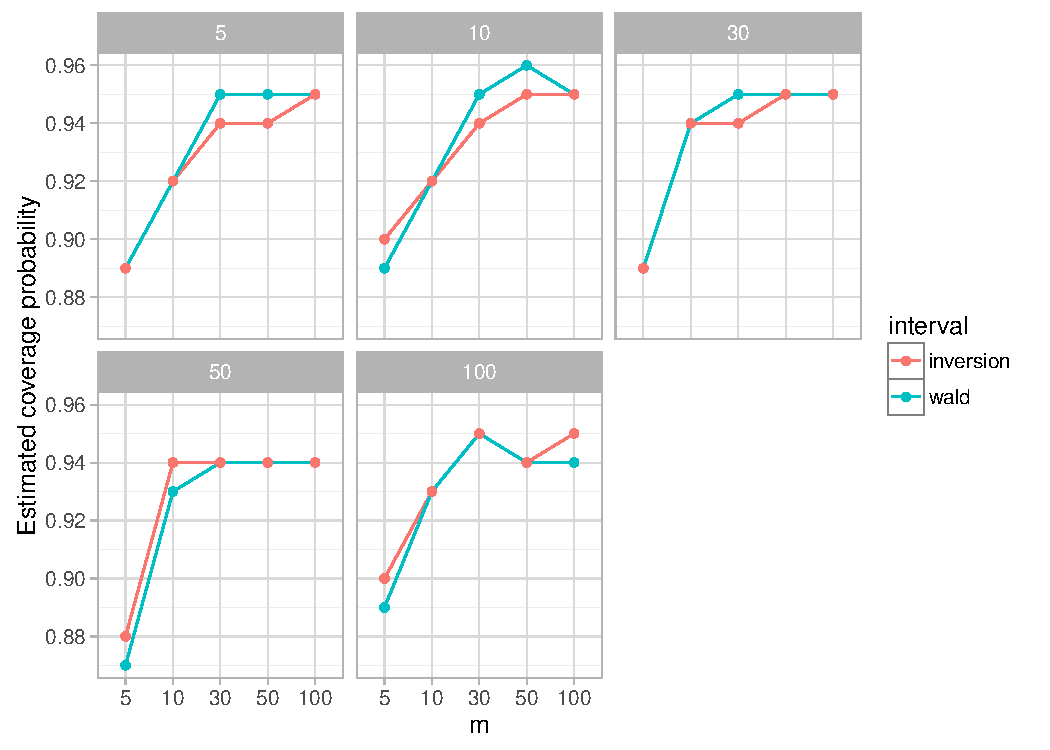
\includegraphics[width=\maxwidth]{figure/simulation-1} \caption[Coverage probability of 95\% confidence intervals for simulated bladder data]{Coverage probability of 95\% confidence intervals for simulated bladder data. The coverage estimates based on the inversion method are colored blue.}\label{fig:simulation}
\end{figure}


\end{knitrout}


%%%%%%%%%%%%%%%%%%%%%%%%%%%%%%%%%%%%%%%%%%%%%%%%%%%%%%%%%%%%%%%%%%%%%%%%%%%%%%%%
\section{Conclusion}
%%%%%%%%%%%%%%%%%%%%%%%%%%%%%%%%%%%%%%%%%%%%%%%%%%%%%%%%%%%%%%%%%%%%%%%%%%%%%%%%

We have discussed a number of confidence interval procedures for statistical calibration in linear models with random coefficients with a single level of grouping.  We have described two \texttt{R} packages for implementing these procedures: \texttt{investr} and \texttt{lme4}.  The \texttt{investr} package can be used for obtaining the asymptotic confidence intervals (i.e., the Wald-based and inversion confidence intervals).  We also showed how the \texttt{lme4} package can be used to obtain calibration intervals based on a parametric bootstrap using the recently added \texttt{bootMer} function.  Future work will likely extend the methods discussed in this paper to more complicated cases such as nonlinear mixed-effects models and multi-level hierarchical models (i.e., more than one grouping variable).


%%%%%%%%%%%%%%%%%%%%%%%%%%%%%%%%%%%%%%%%%%%%%%%%%%%%%%%%%%%%%%%%%%%%%%%%%%%%%%%%
\bibliography{invest-lmm.bib}
%%%%%%%%%%%%%%%%%%%%%%%%%%%%%%%%%%%%%%%%%%%%%%%%%%%%%%%%%%%%%%%%%%%%%%%%%%%%%%%%


%%%%%%%%%%%%%%%%%%%%%%%%%%%%%%%%%%%%%%%%%%%%%%%%%%%%%%%%%%%%%%%%%%%%%%%%%%%%%%%%
\appendix
%%%%%%%%%%%%%%%%%%%%%%%%%%%%%%%%%%%%%%%%%%%%%%%%%%%%%%%%%%%%%%%%%%%%%%%%%%%%%%%%


%%%%%%%%%%%%%%%%%%%%%%%%%%%%%%%%%%%%%%%%%%%%%%%%%%%%%%%%%%%%%%%%%%%%%%%%%%%%%%%%
\section[Inverse estimation in R]{Inverse estimation in \texttt{R}}
\label{sec:R}
%%%%%%%%%%%%%%%%%%%%%%%%%%%%%%%%%%%%%%%%%%%%%%%%%%%%%%%%%%%%%%%%%%%%%%%%%%%%%%%%

Here, we discuss how to implement the previous procedures in the \texttt{R} programming languages.  We discuss two main packages: \texttt{investr} and \texttt{lme4}.  The \texttt{investr} package can be used for obtaining the Wald-based and inversion intervals.  This functionality is demonstrated over the next two sections.  The \texttt{lme4} package is a popular package for fitting linear, generalized linear, and nonlinear mixed models. Recently, however, the \texttt{lme4} package creators have added functionality for model-based parametric bootstrapping.  In Section~\ref{sec:lme4}, we demonstrate the potential of this new functionality by applying our parametric bootstrap algorithm to the bladder volume data discussed earlier.

\subsection[The investr package]{The \texttt{investr} package}

The \texttt{R} package \texttt{investr} facilitates calibration/inverse estimation with linear and nonlinear regression models.  The main function, \texttt{invest}, can be used for inverse estimation of $x_0$ given an observed response $y_0$.  More recently, the package has been updated to also handle objects of class \texttt{lme} from the \texttt{nlme} package.  Current functionality includes both the Wald-based and inversion methods outlined in Sections \ref{sec:wald}-\ref{sec:inversion}.  The code for the package is hosted on GitHub at \url{https://github.com/bgreenwell/investr}, but the latest stable release can be found on CRAN at \url{https://CRAN.R-project.org/package=investr}.

% \begin{table}[!htb]
% \begin{tabular}{lp{12cm}}
%   \toprule
%   Argument    & Description \\
%   \midrule
%   \texttt{object}        & An object that inherits from class \texttt{"lm"}, \texttt{"glm"}, \texttt{"nls"}, or \texttt{"lme"} \\
%   \texttt{y0}            & The value of the observed response(s) or specified value of the \\ & mean response. For \texttt{"glm"} objects, \texttt{y0} should be on scale of the \\ & response variable. \\
%   \texttt{interval}      & The type of interval required. Currently, only \texttt{"inversion"}, \\ & \texttt{"Wald"}, \texttt{"percentile"}, and \texttt{"none"} are supported. \\
%   \texttt{level}         & A numeric scalar between 0 and 1 giving the confidence level \\ & for the interval to be calculated. The default is \texttt{0.95}. \\
%   \texttt{lower}         & The lower endpoint of the interval to be searched. \\
%   \texttt{upper} 				 & The upper endpoint of the interval to be searched. \\
%   \texttt{q1}            & Optional lower cutoff to be used in forming \\ & confidence intervals. Only used when object inherits from class \\ & \texttt{"lme"}. Defaults to \texttt{stats::qnorm((1+level)/2)}. \\
%   \texttt{q2}            & Optional upper cutoff to be used in forming \\ & confidence intervals. Only used when object inherits from class \\ & \texttt{"lme"}. Defaults to \texttt{stats::qnorm((1-level)/2)}. \\
%   \bottomrule
% \end{tabular}
% \caption{Main arguments for the \texttt{invest} function. \label{tab:invest}}
% \end{table}

Returning to the bladder volume example, suppose we obtained an ultrasound measurement from a new patient for which $\texttt{HD}^{3/2} = 500$ (that's roughly 63 on the original scale).  What is the true volume of fluid ($x_0$) in the patients bladder?  We can estimate the true volume and form an approximate 95\% confidence interval using the methods discussed previously.  The point estimate is simply given by
\[
  \widehat{x}_0 = \frac{500 + 53.83164}{69.09491} = 8.0155 \text{ (cl)}.
\]
This estimate can be obtained in \texttt{R} as follows:
\begin{knitrout}
\definecolor{shadecolor}{rgb}{0.969, 0.969, 0.969}\color{fgcolor}\begin{kframe}
\begin{alltt}
\hlkwd{library}\hlstd{(investr)}
\hlkwd{invest}\hlstd{(fit.lme,} \hlkwc{y0} \hlstd{=} \hlnum{500}\hlstd{,} \hlkwc{interval} \hlstd{=} \hlstr{"none"}\hlstd{)}
\end{alltt}
\begin{verbatim}
## [1] 8.02
\end{verbatim}
\end{kframe}
\end{knitrout}
\texttt{invest} relies on the root finding function \texttt{uniroot} from the \texttt{stats} package to solve the equation $f\left(x; \widehat{\bm{\beta}}\right) - y_0 = 0$ numerically for $x$.  

When \texttt{interval = "Wald"}, an asymptotic $100(1-\alpha)\%$ confidence interval (where $\alpha$ is equal to \texttt{1 - level}) for $x_0$ is calculated according to Equation~\eqref{eqn:wald}. The standard error is computed using a First-order Taylor series approximation by calling the \texttt{stats} function \texttt{numericDeriv} to numerically evaluate the gradient of $\widehat{x}_0$ as a function of $y_0$ and the fixed-effects $\widehat{\bm{\beta}}$.
\begin{knitrout}
\definecolor{shadecolor}{rgb}{0.969, 0.969, 0.969}\color{fgcolor}\begin{kframe}
\begin{alltt}
\hlkwd{invest}\hlstd{(fit.lme,} \hlkwc{y0} \hlstd{=} \hlnum{500}\hlstd{,} \hlkwc{interval} \hlstd{=} \hlstr{"Wald"}\hlstd{)}
\end{alltt}
\begin{verbatim}
## estimate    lower    upper       se 
##     8.02     4.18    11.85     1.95
\end{verbatim}
\end{kframe}
\end{knitrout}

Alternatively, one can use the very useful \texttt{deltaMethod} function from the \texttt{car} package to obtain \texttt{se}:
\begin{knitrout}
\definecolor{shadecolor}{rgb}{0.969, 0.969, 0.969}\color{fgcolor}\begin{kframe}
\begin{alltt}
\hlkwd{library}\hlstd{(car)}  \hlcom{# assuming package car is already installed}
\hlstd{params} \hlkwb{<-} \hlkwd{c}\hlstd{(}\hlkwd{fixef}\hlstd{(fit.lme),} \hlnum{500}\hlstd{)}
\hlstd{covmat} \hlkwb{<-} \hlkwd{diag}\hlstd{(}\hlnum{3}\hlstd{)}  \hlcom{# set up var/cov matrix}
\hlstd{covmat[}\hlnum{1}\hlopt{:}\hlnum{2}\hlstd{,} \hlnum{1}\hlopt{:}\hlnum{2}\hlstd{]} \hlkwb{<-} \hlkwd{vcov}\hlstd{(fit.lme)}  \hlcom{# fixed-effects var/cov matrix}
\hlstd{covmat[}\hlnum{3}\hlstd{,} \hlnum{3}\hlstd{]} \hlkwb{<-}  \hlnum{17572.35}  \hlcom{# VAR[Y_0]}
\hlkwd{names}\hlstd{(params)} \hlkwb{<-} \hlkwd{c}\hlstd{(}\hlstr{"b0"}\hlstd{,} \hlstr{"b1"}\hlstd{,} \hlstr{"y0"}\hlstd{)}
\hlkwd{deltaMethod}\hlstd{(params,} \hlkwc{g} \hlstd{=} \hlstr{"(y0 - b0)/b1"}\hlstd{,}  \hlkwc{vcov.} \hlstd{= covmat)}\hlopt{$}\hlstd{SE}
\end{alltt}
\begin{verbatim}
## [1] 1.95
\end{verbatim}
\end{kframe}
\end{knitrout}
The only drawback here is that \texttt{deltaMethod} relies on the \texttt{stats} package symbolic differentiation function \texttt{D}; hence, $\widehat{x}_0 = f^{-1}\left(y_0; \widehat{\bm{\beta}}\right)$ has to be obtainable in closed-form.

To obtain the inversion interval \eqref{eqn:inversion}, we set \texttt{interval = "inversion"} (the default) in the call to invest:
\begin{knitrout}
\definecolor{shadecolor}{rgb}{0.969, 0.969, 0.969}\color{fgcolor}\begin{kframe}
\begin{alltt}
\hlkwd{invest}\hlstd{(fit.lme,} \hlkwc{y0} \hlstd{=} \hlnum{500}\hlstd{,} \hlkwc{interval} \hlstd{=} \hlstr{"inversion"}\hlstd{)}
\end{alltt}
\begin{verbatim}
## estimate    lower    upper 
##     8.02     4.23    11.92
\end{verbatim}
\end{kframe}
\end{knitrout}
Essentially, \texttt{invest} finds the lower and upper inversion confidence limits \eqref{eqn:inversion} by solving the equations
\begin{equation*}
  Q_I - z_{\alpha/2} = 0 \quad \text{and} \quad Q_I - z_{1-\alpha/2} = 0
\end{equation*}
numerically for $x$ using \texttt{uniroot}. To use the quantiles from a $t$~distribution instead (see Section~\ref{sec:inversion}), we can supply them via the arguments \texttt{q1} and \texttt{q2}:
\begin{knitrout}
\definecolor{shadecolor}{rgb}{0.969, 0.969, 0.969}\color{fgcolor}\begin{kframe}
\begin{alltt}
\hlstd{tvals} \hlkwb{<-} \hlkwd{qt}\hlstd{(}\hlkwd{c}\hlstd{(}\hlnum{0.025}\hlstd{,} \hlnum{0.975}\hlstd{),} \hlkwc{df} \hlstd{=} \hlkwd{nrow}\hlstd{(bladder)} \hlopt{-} \hlnum{1}\hlstd{)}
\hlkwd{invest}\hlstd{(fit.lme,} \hlkwc{y0} \hlstd{=} \hlnum{500}\hlstd{,} \hlkwc{q1} \hlstd{= tvals[}\hlnum{1L}\hlstd{],} \hlkwc{q2} \hlstd{= tvals[}\hlnum{2L}\hlstd{])}
\end{alltt}
\begin{verbatim}
## estimate    lower    upper 
##     8.02     4.20    11.95
\end{verbatim}
\end{kframe}
\end{knitrout}
Being able to specify the arguments \texttt{q1} and \texttt{q2} will also be useful when implementing the bootstrap adjusted inversion interval described in Section~\ref{sec:parboot}


%%%%%%%%%%%%%%%%%%%%%%%%%%%%%%%%%%%%%%%%%%%%%%%%%%%%%%%%%%%%%%%%%%%%%%%%%%%%%%%%
\subsection[Using the lme4 package]{Using the \texttt{lme4} package}
\label{sec:lme4}
%%%%%%%%%%%%%%%%%%%%%%%%%%%%%%%%%%%%%%%%%%%%%%%%%%%%%%%%%%%%%%%%%%%%%%%%%%%%%%%%

Implementation of the parametric bootstrap algorithm in Figure~\ref{fig:parboot} is relatively straight forward using the new \texttt{bootMer} function from the well-known \texttt{R} package \texttt{lme4} \citep{bates-lme4-2014} in conjunction with the \texttt{boot} package.
\begin{knitrout}
\definecolor{shadecolor}{rgb}{0.969, 0.969, 0.969}\color{fgcolor}\begin{kframe}
\begin{alltt}
\hlkwd{install.packages}\hlstd{(}\hlstr{"investr"}\hlstd{,} \hlstr{"lme4"}\hlstd{)}
\end{alltt}
\end{kframe}
\end{knitrout}

Since we will be using the \texttt{lme4} package, we need to refit the model using the \texttt{lmer} function:
\begin{knitrout}
\definecolor{shadecolor}{rgb}{0.969, 0.969, 0.969}\color{fgcolor}\begin{kframe}
\begin{alltt}
\hlkwd{library}\hlstd{(lme4)}
\hlstd{fit.lmer} \hlkwb{<-} \hlkwd{lmer}\hlstd{(HD} \hlopt{^} \hlstd{(}\hlnum{3} \hlopt{/} \hlnum{2}\hlstd{)} \hlopt{~} \hlstd{volume} \hlopt{+} \hlstd{(}\hlnum{0} \hlopt{+} \hlnum{1} \hlopt{|} \hlstd{subject)} \hlopt{+}
                           \hlstd{(}\hlnum{0} \hlopt{+} \hlstd{volume} \hlopt{|} \hlstd{subject),} \hlkwc{data} \hlstd{= bladder)}
\end{alltt}
\end{kframe}
\end{knitrout}
Theoretically, the parameter estimates from this model should be the same as those from \texttt{fit.lme}; however, there are likely to be small numerical differences between the two.  For this reason, let us re-estimate $\widehat{x}_0$ using \texttt{fit.lmer}.  Since \texttt{invest} does not work on objects of class \texttt{"lmer"}, we have to do things manually:
\begin{knitrout}
\definecolor{shadecolor}{rgb}{0.969, 0.969, 0.969}\color{fgcolor}\begin{kframe}
\begin{alltt}
\hlstd{fe} \hlkwb{<-} \hlkwd{unname}\hlstd{(}\hlkwd{fixef}\hlstd{(fit.lmer))}  \hlcom{# fixed-effects}
\hlstd{(x0.est} \hlkwb{<-} \hlstd{(}\hlnum{500} \hlopt{-} \hlstd{fe[}\hlnum{1}\hlstd{])} \hlopt{/} \hlstd{fe[}\hlnum{2}\hlstd{])}
\end{alltt}
\begin{verbatim}
## [1] 8.02
\end{verbatim}
\end{kframe}
\end{knitrout}
Also, for convenience, we define the following function which estimates $\VAR\left[\mathcal{Y}|x\right] = \sigma_0^2 + x^2\sigma_1^2 + \sigma^2$ for a given value of $x$:
\begin{knitrout}
\definecolor{shadecolor}{rgb}{0.969, 0.969, 0.969}\color{fgcolor}\begin{kframe}
\begin{alltt}
\hlstd{varY} \hlkwb{<-} \hlkwa{function}\hlstd{(}\hlkwc{object}\hlstd{,} \hlkwc{x}\hlstd{) \{}
  \hlstd{vc} \hlkwb{<-} \hlkwd{as.data.frame}\hlstd{(lme4}\hlopt{::}\hlkwd{VarCorr}\hlstd{(object))}\hlopt{$}\hlstd{vcov}
  \hlstd{vc[}\hlnum{1}\hlstd{]} \hlopt{+} \hlstd{vc[}\hlnum{2}\hlstd{]}\hlopt{*}\hlstd{x}\hlopt{^}\hlnum{2} \hlopt{+} \hlstd{vc[}\hlnum{3}\hlstd{]}
\hlstd{\}}
\end{alltt}
\end{kframe}
\end{knitrout}
For example, to estimate $\sigma_0^2 = \widehat{\VAR}\left[\mathcal{Y}_0\right]$, we have \texttt{varY(fit.lmer, x = x0.est)}, which gives \ensuremath{1.757\times 10^{4}}, the same value used in the previous section.

Although we could easily compute all the bootstrap intervals previously discussed in one call to \texttt{bootMer} and \texttt{boot.ci}, we will discuss and compute each interval separately.

The following snippet of code generates $R = 9999$ bootstrap replicates of $\widehat{x}_0$, $Q_W$, and $Q_I$ according to the algorithm in Figure~\ref{fig:parboot}:
\begin{knitrout}
\definecolor{shadecolor}{rgb}{0.969, 0.969, 0.969}\color{fgcolor}\begin{kframe}
\begin{alltt}
\hlstd{pboot} \hlkwb{<-} \hlkwd{bootMer}\hlstd{(fit.lmer,} \hlkwc{nsim} \hlstd{=} \hlnum{9}\hlstd{,} \hlkwc{seed} \hlstd{=} \hlnum{105}\hlstd{,} \hlkwc{FUN} \hlstd{=} \hlkwa{function}\hlstd{(}\hlkwc{.}\hlstd{) \{}

  \hlcom{# Point estimate}
  \hlstd{var.Y0.boot} \hlkwb{<-} \hlkwd{varY}\hlstd{(.,} \hlkwc{x} \hlstd{= x0.est)}  \hlcom{# VAR[Y0]}
  \hlstd{fe.boot} \hlkwb{<-} \hlkwd{unname}\hlstd{(}\hlkwd{fixef}\hlstd{(.))}  \hlcom{# fixed-effects}
  \hlkwa{if} \hlstd{(}\hlkwd{all}\hlstd{(}\hlkwd{getME}\hlstd{(.,} \hlstr{"y"}\hlstd{)} \hlopt{==} \hlstd{bladder}\hlopt{$}\hlstd{HD} \hlopt{^} \hlstd{(}\hlnum{3} \hlopt{/} \hlnum{2}\hlstd{))) \{}
    \hlstd{y0.boot} \hlkwb{<-} \hlnum{500}
  \hlstd{\}} \hlkwa{else} \hlstd{\{}
    \hlstd{y0.boot} \hlkwb{<-} \hlkwd{rnorm}\hlstd{(}\hlnum{1}\hlstd{,} \hlnum{500}\hlstd{,} \hlkwd{sqrt}\hlstd{(var.Y0.boot))}
  \hlstd{\}}
  \hlstd{x0.boot} \hlkwb{<-} \hlstd{(y0.boot} \hlopt{-} \hlstd{fe.boot[}\hlnum{1}\hlstd{])} \hlopt{/} \hlstd{fe.boot[}\hlnum{2}\hlstd{]}

  \hlcom{# Approximate variance}
  \hlstd{covmat} \hlkwb{<-} \hlkwd{diag}\hlstd{(}\hlnum{3}\hlstd{)}
  \hlstd{covmat[}\hlnum{1L}\hlopt{:}\hlnum{2L}\hlstd{,} \hlnum{1L}\hlopt{:}\hlnum{2L}\hlstd{]} \hlkwb{<-} \hlkwd{as.matrix}\hlstd{(}\hlkwd{vcov}\hlstd{(.))}
  \hlstd{covmat[}\hlnum{3L}\hlstd{,} \hlnum{3L}\hlstd{]} \hlkwb{<-}  \hlstd{var.Y0.boot}
  \hlstd{params} \hlkwb{<-} \hlkwd{c}\hlstd{(}\hlstr{"b0"} \hlstd{= fe.boot[}\hlnum{1}\hlstd{],}
              \hlstr{"b1"} \hlstd{= fe.boot[}\hlnum{2}\hlstd{],}
              \hlstr{"y0"} \hlstd{= y0.boot)}
  \hlstd{dm} \hlkwb{<-} \hlstd{car}\hlopt{::}\hlkwd{deltaMethod}\hlstd{(params,} \hlkwc{g} \hlstd{=} \hlstr{"(y0 - b0) / b1"}\hlstd{,}  \hlkwc{vcov.} \hlstd{= covmat)}
  \hlstd{var.x0.boot} \hlkwb{<-} \hlstd{dm}\hlopt{$}\hlstd{SE} \hlopt{^} \hlnum{2}

  \hlcom{# Approximate predictive pivot}
  \hlstd{mu0.boot} \hlkwb{<-}  \hlkwd{as.numeric}\hlstd{(}\hlkwd{crossprod}\hlstd{(fe.boot,} \hlkwd{c}\hlstd{(}\hlnum{1}\hlstd{, x0.est)))}
  \hlstd{var.mu0.boot} \hlkwb{<-} \hlkwd{t}\hlstd{(}\hlkwd{c}\hlstd{(}\hlnum{1}\hlstd{, x0.est))} \hlopt
    \hlkwd{as.matrix}\hlstd{(}\hlkwd{vcov}\hlstd{(.))} \hlopt \hlkwd{c}\hlstd{(}\hlnum{1}\hlstd{, x0.est)}
  \hlstd{QI.boot} \hlkwb{<-} \hlstd{(y0.boot} \hlopt{-} \hlstd{mu0.boot)} \hlopt{/} \hlkwd{sqrt}\hlstd{(var.Y0.boot} \hlopt{+} \hlstd{var.mu0.boot)}

  \hlcom{# Return values}
  \hlkwd{c}\hlstd{(x0.boot, var.x0.boot, QI.boot)}

\hlstd{\})}
\end{alltt}
\end{kframe}
\end{knitrout}
The \texttt{bootMer} function returns an object of class \texttt{boot} which can then be processed via the \texttt{boot} package to obtain the various bootstrap confidence intervals discussed earlier.  A basic summary of \texttt{pboot} is given by
\begin{knitrout}
\definecolor{shadecolor}{rgb}{0.969, 0.969, 0.969}\color{fgcolor}\begin{kframe}
\begin{alltt}
\hlkwd{library}\hlstd{(boot)}  \hlcom{# load boot package}
\hlkwd{summary}\hlstd{(pboot)}
\end{alltt}
\begin{verbatim}
##      R original bootBias bootSE bootMed
## 1 9999     8.02 -0.00219  1.974  8.0186
## 2 9999     1.95 -0.00330  0.256  1.9417
## 3 9999     0.00 -0.00810  1.004  0.0016
\end{verbatim}
\end{kframe}
\end{knitrout}
The estimated standard error and bias of $\widehat{x}_0$, based on \texttt{R = 9999} bootstrap replicates, are 1.974 and \ensuremath{-0.003}, respectively.  The original estimate $\widehat{x}_0$ and the median of the bootstrap replicates are also given in the first row of the summary.  A graphical summary of the bootstrap simulation is given in Figure~\ref{fig:boot-plots}.  These graphs indicate that the sampling distributions of $\widehat{x}_0$, $Q_W$, and $Q_I$ are all approximately normal; hence, we would expect the bootstrap confidence intervals to be similar to the asymptotic methods based on the normal distribution discussed in Sections~\ref{sec:wald}-\ref{sec:inversion}.
\begin{knitrout}
\definecolor{shadecolor}{rgb}{0.969, 0.969, 0.969}\color{fgcolor}\begin{figure}[!htb]
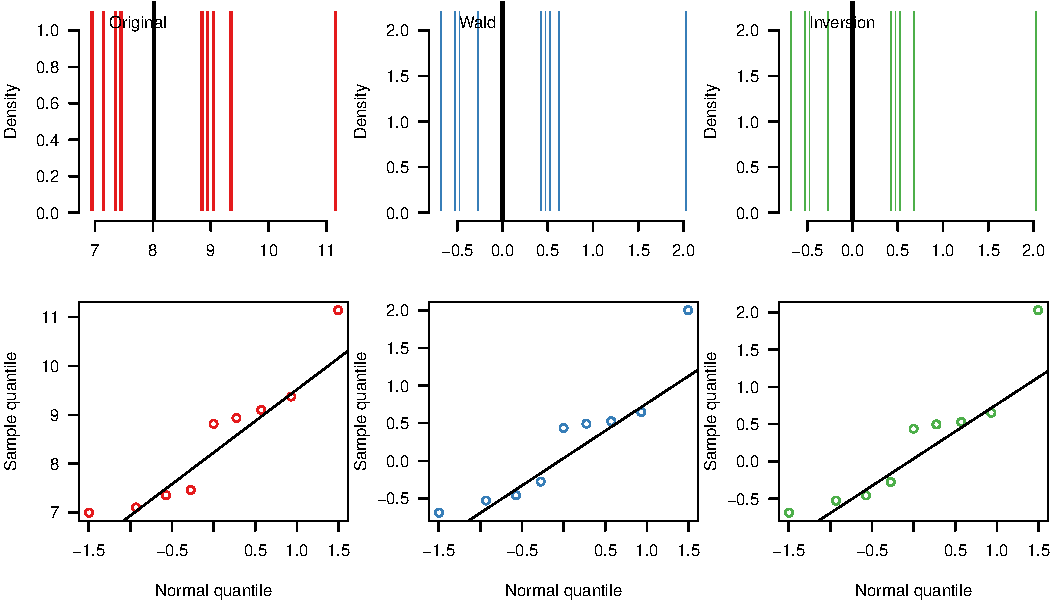
\includegraphics[width=\linewidth]{figure/boot-plots-1} \caption[Graphical summary of bootstrap replicates]{Graphical summary of bootstrap replicates. $R = 9,999$ bootstrap replicates of $\widehat{x}_0$ (left), $Q_W$ (middle), and $Q_I$ (right).}\label{fig:boot-plots}
\end{figure}


\end{knitrout}
To obtain the percentile and studentized $t$ intervals (see Sections~\ref{sec:percentile}-\ref{sec:student}), we can use the \texttt{boot} package function \texttt{boot.ci}:
\begin{knitrout}
\definecolor{shadecolor}{rgb}{0.969, 0.969, 0.969}\color{fgcolor}\begin{kframe}
\begin{alltt}
\hlkwd{boot.ci}\hlstd{(pboot,} \hlkwc{type} \hlstd{=} \hlkwd{c}\hlstd{(}\hlstr{"norm"}\hlstd{,} \hlstr{"perc"}\hlstd{,} \hlstr{"stud"}\hlstd{))}
\end{alltt}
\begin{verbatim}
## BOOTSTRAP CONFIDENCE INTERVAL CALCULATIONS
## Based on 9999 bootstrap replicates
## 
## CALL : 
## boot.ci(boot.out = pboot, type = c("norm", "perc", "stud"))
## 
## Intervals : 
## Level      Normal            Studentized          Percentile     
## 95%   ( 4.15, 11.89 )   ( 4.25, 11.95 )   ( 4.05, 11.91 )  
## Calculations and Intervals on Original Scale
\end{verbatim}
\end{kframe}
\end{knitrout}
For comparison, we also included the option to compute a bootstrap normal-approximation confidence interval.  This interval has the form
\[
  \left( \widehat{x}_0- \texttt{bootBias} \right) \pm z_{\alpha/2}\texttt{bootSE}
\]
where \texttt{bootBias} and \texttt{bootSE} can be found in the first row of \texttt{summary(pboot)}.  In other words, it is just a Wald-type interval that uses a bias-corrected estimate of $x_0$, along with a bootstrap estimate of the standard error of $\widehat{x}_0$.  While this may be more accurate than the ordinary Wald-based interval \eqref{eqn:wald}, it may still not perform well in small sample sizes because of the strict normality assumption.  In this example, however, normality does not appear to be an issue.

The bootstrap adjusted inversion interval can be computed as easily as the ordinary inversion interval, except we need to supply \texttt{invest} with the estimated quantiles $\widehat{F}_{Q_I}\left(0.025\right)$ and $\widehat{F}_{Q_I}\left(0.975\right)$:
\begin{knitrout}
\definecolor{shadecolor}{rgb}{0.969, 0.969, 0.969}\color{fgcolor}\begin{kframe}
\begin{alltt}
\hlstd{QI.boot} \hlkwb{<-} \hlstd{pboot}\hlopt{$}\hlstd{t[,} \hlnum{3}\hlstd{]}  \hlcom{# bootsrap replicates of Q_I}
\hlstd{qvals} \hlkwb{<-} \hlkwd{quantile}\hlstd{(QI.boot,} \hlkwd{c}\hlstd{(}\hlnum{0.025}\hlstd{,} \hlnum{0.975}\hlstd{))}  \hlcom{# sample quantiles}
\hlkwd{invest}\hlstd{(fit.lme,} \hlkwc{y0} \hlstd{=} \hlnum{500}\hlstd{,} \hlkwc{q1} \hlstd{= qvals[}\hlnum{1}\hlstd{],} \hlkwc{q2} \hlstd{= qvals[}\hlnum{2}\hlstd{])}
\end{alltt}
\begin{verbatim}
## estimate    lower    upper 
##     8.02     4.28    12.02
\end{verbatim}
\end{kframe}
\end{knitrout}

\end{document}
